\newpage
\subsection{Caso d'uso UC6: Ricerca e iscrizione questionario}
\label{UC6}
\begin{figure}[h]
\centering
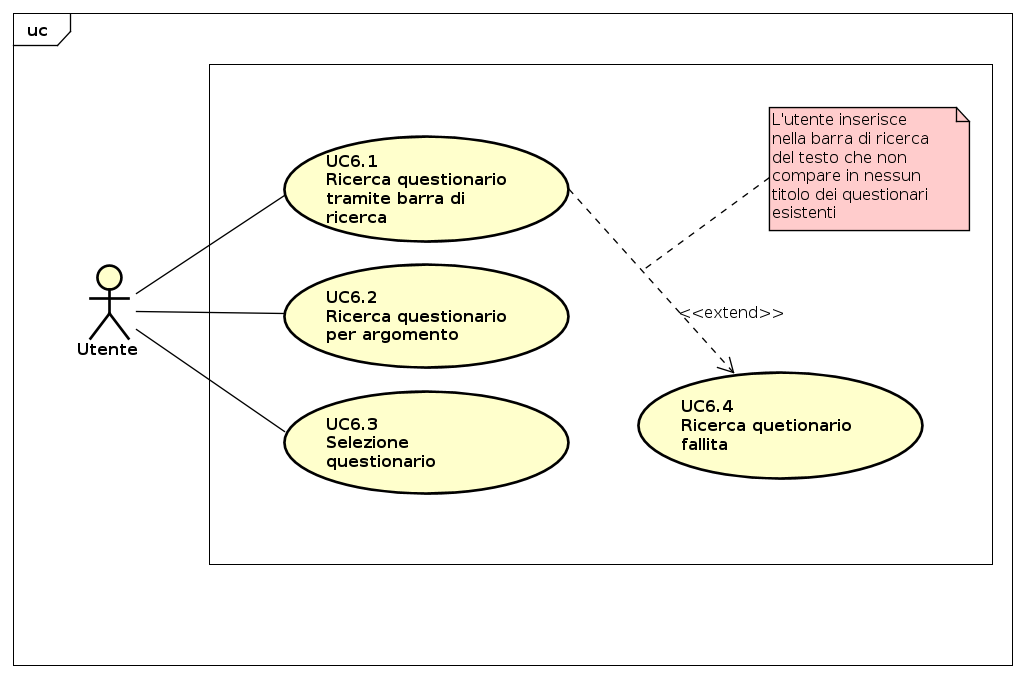
\includegraphics[scale=0.5,keepaspectratio]{UML/UC6.png}
\caption{UC6: Ricerca e iscrizione questionario}
\end{figure}
\FloatBarrier
\begin{itemize}
\item\textbf{Attori}: utente autenticato, utente autenticato pro;
\item\textbf{Descrizione}: nella schermata principale qualsiasi attore che voglia iscriversi ad un questionario può ricercarlo attraverso la barra di ricerca. L'attore, per poter compilare un questionario, dovrà poi iscriversi al questionario selezionato;	
\item\textbf{Precondizione}: l'attore si trova nella pagina principale dell'applicazione;
\item\textbf{Postcondizione}: l'attore si è iscritto al questionario che vuole compilare;
\item\textbf{Scenario principale}:
\begin{enumerate}
\item L'attore può cercare un questionario tramite barra di ricerca (UC6.1);
\item L'attore può iscriversi al questionario scelto (UC6.2).
\end{enumerate}
\item\textbf{Estensioni}: ricerca questionario fallita (UC6.3);
\item\textbf{Scenari Alternativi}: l'attore ricerca un questionario che non esiste. 
\end{itemize}

\subsubsection{Caso d'uso UC6.1: Ricerca questionario tramite barra di ricerca}
\label{UC6.1}
\begin{itemize}
\item\textbf{Attori}: utente autenticato, utente autenticato pro;
\item\textbf{Descrizione}: all'interno della pagina principale dell'applicazione è presente una barra di ricerca dove l'attore può cercare i questionari;
\item\textbf{Precondizione}: l'attore si trova nella pagina principale dell'applicazione;
\item\textbf{Postcondizione}: l'attore visualizza i questionari che contengono il testo scritto nella barra di ricerca;
\item\textbf{Scenario principale}: l'attore utilizza la barra di ricerca per cercare un questionario.
\end{itemize}

\subsubsection{Caso d'uso UC6.2: Iscrizione questionario}
\label{UC6.2}
\begin{figure}[h]
\centering
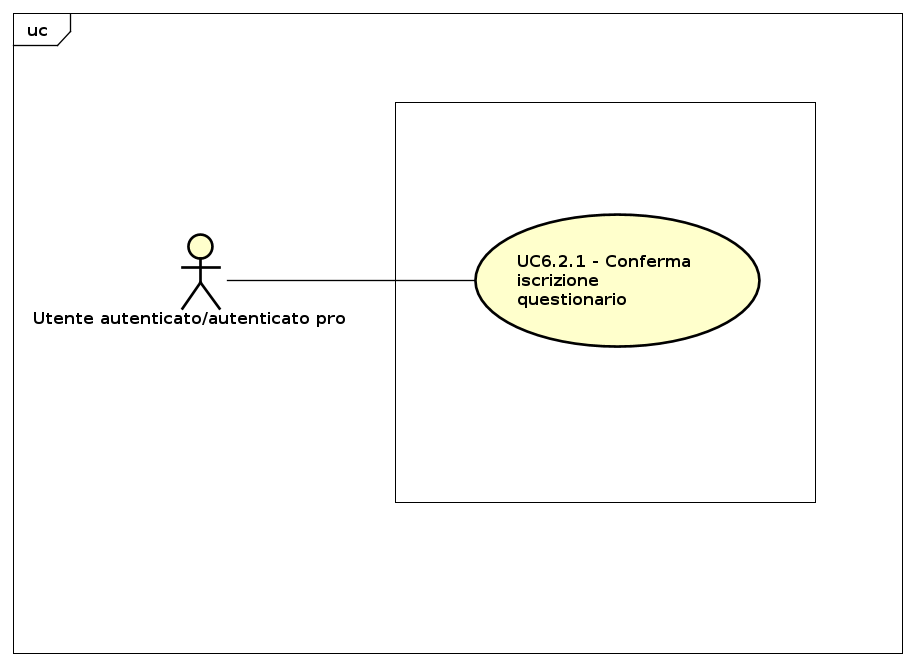
\includegraphics[scale=0.5,keepaspectratio]{UML/UC6_2.png}
\caption{UC6.2: Iscrizione questionario}
\end{figure}
\FloatBarrier
\begin{itemize}
\item\textbf{Attori}: utente autenticato, utente autenticato pro;
\item\textbf{Descrizione}: l'attore dopo aver scelto un questionario, per iniziare a compilarlo, può iscriversi;
\item\textbf{Precondizione}: l'attore ha scelto il questionario che vuole svolgere;
\item\textbf{Postcondizione}: l'attore si è iscritto al questionario scelto;
\item\textbf{Scenario principale}: 
\begin{enumerate}
\item L'attore può confermare l'iscrizione al questionario (UC6.2.1).
\end{enumerate}
\item\textbf{Scenari alternativi}: l'attore cambia idea sul questionario al quale vuole iscriversi e annulla l'operazione tornando alla schermata precedente.
\end{itemize}

\subsubsection{Caso d'uso UC6.2.1: Conferma iscrizione questionario}
\label{UC6.2.1}
\begin{itemize}
\item\textbf{Attori}: utente autenticato, utente autenticato pro;
\item\textbf{Descrizione}: l'attore conferma l'iscrizione al questionario, potendo così procedere con la compilazione;
\item\textbf{Precondizione}: l'attore si è iscritto ad un questionario;
\item\textbf{Postcondizione}: l'attore ha confermato l'iscrizione al questionario;
\item\textbf{Scenario principale}: l'attore conferma di voler compilare il questionario a cui si è iscritto.
\end{itemize}

\subsubsection{Caso d'uso UC6.3: Ricerca questionario fallita}
\label{UC6.3}
\begin{itemize}
\item\textbf{Attori}: utente autenticato, utente autenticato pro;
\item\textbf{Descrizione}: l'attore ha inserito nella barra di ricerca del testo che non compare in nessuno dei questionari esistenti;
\item\textbf{Precondizione}: l'attore ha utilizzato la barra di ricerca per cercare un questionario che non esiste;
\item\textbf{Postcondizione}: il sistema avvisa l'attore dell'errore verificatosi tramite un opportuno messaggio;
\item\textbf{Scenario principale}: l'attore visualizza un messaggio che lo avvisa del mancato ritrovamento di questionari.
\end{itemize}